%
% Draft  document appendixA.tex
% Testing if Fn with IntGpDens and FollperGp improved classification
%
 
\documentclass[titlepage]{article}  % Latex2e
\usepackage{graphicx,lscape,subfigure}
\usepackage{bm}
\usepackage{textcomp}
\usepackage[flushleft]{threeparttable}
 
\begin{document} 
\appendix
\section{Appendix B: Testing whether a fleece density  would improve classification if augmented with follicle spatial distribution information}
 
Perhaps density would be a better aid to classifying crimp types if we could augment it with information about the spatial distribution of follicles. To investigate this we will add the variables "IntGpDens",  "FollperGp" and "FollGpArea" to the classification analyses.  "IntGpDens" or intra-group-density is the number of follicles per group ("FollperGp") divided by follicle group area ("FollGpArea").

So we now make up a set of 14 traits - 10 on-sheep traits, Fn, and the three spatial traits IntGpDens, FollperGp, and FollGpArea.
\begin{verbatim}
> form.14 <- formula(CrimpType ~ StapMaxD + StapMinD + StapArea + CompEx +
     Softness + Lustre + Whiteness + PeelScore + CrimpFreq + Zigzag +
     Fn + IntGpDens  + FollperGp + FollGpArea)
> 
and then run the recursive partitioning algorithm on 14 traits and get
\begin{verbatim}
> rpart.14 <- rpart(form.14,jan20sf2.df)
> rpart.14
n= 306 

node), split, n, loss, yval, (yprob)
      * denotes terminal node

 1) root 306 148 stretched (0.516339869 0.091503268 0.392156863)  
   2) CompEx< 3.5 204  64 stretched (0.686274510 0.132352941 0.181372549)  
     4) Zigzag>=1.5 178  47 stretched (0.735955056 0.061797753 0.202247191)  
       8) Zigzag< 3.5 158  35 stretched (0.778481013 0.069620253 0.151898734)  
        16) IntGpDens< 98.3 130  20 stretched (0.846153846 0.053846154 0.100000000) *
        17) IntGpDens>=98.3 28  15 stretched (0.464285714 0.142857143 0.392857143)  
          34) StapMinD>=1.65 19   6 stretched (0.684210526 0.157894737 0.157894737) *
          35) StapMinD< 1.65 9   1 unfolded (0.000000000 0.111111111 0.888888889) *
       9) Zigzag>=3.5 20   8 unfolded (0.400000000 0.000000000 0.600000000)  
        18) StapMinD>=1.85 11   4 stretched (0.636363636 0.000000000 0.363636364) *
        19) StapMinD< 1.85 9   1 unfolded (0.111111111 0.000000000 0.888888889) *
     5) Zigzag< 1.5 26  10 unaligned (0.346153846 0.615384615 0.038461538) *
   3) CompEx>=3.5 102  19 unfolded (0.176470588 0.009803922 0.813725490)  
     6) IntGpDens< 61.8 9   3 stretched (0.666666667 0.000000000 0.333333333) *
     7) IntGpDens>=61.8 93  13 unfolded (0.129032258 0.010752688 0.860215054) *
> 
\end{verbatim}
 So now we have something diffrent - it is using IntGpDens, but not Fn, and it is not using FollperGp or FollGpArea.

If we look at the 'importance rating' of variables now we get
\begin{verbatim}
> rpart.14$variable.importance
    CompEx     Zigzag   StapArea   StapMaxD  IntGpDens   StapMinD  PeelScore 
49.2260711 24.6984711 14.1271202 13.4629421 12.3272316 10.5643351  9.9092431 
        Fn     Lustre  CrimpFreq FollGpArea  FollperGp 
 9.3268283  3.8188483  2.0452520  1.5649231  0.5868462 
> 
\end{verbatim}
 we see IntGpDens is position 5, but the other two ( FollGpArea and FollperGp) are dead last.

If we construct a confusion matrix we get
\begin{verbatim}
> table(predicted=rpred(prpart.14),actual=ct306)
           actual
predicted   stretched unaligned unfolded
  stretched       136        10       23
  unaligned         9        16        1
  unfolded         13         2       96
> 
\end{verbatim}
which is a little better than the original 10 trait case. We now have 248 correctly classified, so the success rate is $248/306==.81$, which is a little better than the 0.78 success rate achieved with 10 on-sheep traits.

A plot of the classification tree is shown in Figure~\ref{fig:rpart14}
%\documentclass{article}
%\usepackage{graphicx,subfigure}
%\begin{document}

\begin{figure}[!h]
  \centering
  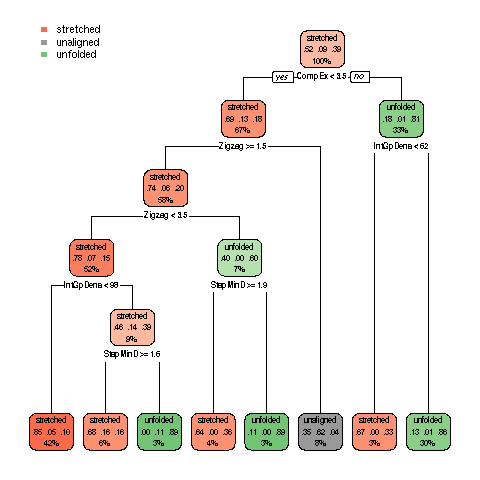
\includegraphics[width=1.1\textwidth]{figrpart14.png}
  \caption{A binary tree produced by allowing splits on 14 traits - the 10 on-sheep traits plus Fn, IntGpDens, FollperGp, and FollGpArea}
  \label{fig:rpart14}
\end{figure}

%\end{document}


We see that it is using IntGpDens in two ways. First to split low IntGpDens animals out of the unfolded class, then at the bottom to split some high IntGpDens animals out of the stretched class. 

The disappoiting thing is that there does not seem to be any interplay between 
IntGpDens and Fn - it is not using it to refine the meaning of Fn, it is using it in its own right.

Lets see if we can improve on that with discriminant functions. We run a linear discriminant analysis using all 14 traits and get
\begin{verbatim}
> lda.14 <- lda(form.14,jan20sf2.df)
> lda.14
Call:
lda(form.14, data = jan20sf2.df)

Prior probabilities of groups:
stretched unaligned  unfolded 
0.5138889 0.0937500 0.3923611 

Group means:
          StapMaxD StapMinD  StapArea   CompEx Softness   Lustre Whiteness
stretched 4.579054 2.240541 10.689189 2.885135 3.506757 3.378378  3.317568
unaligned 6.618519 2.966667 20.937037 1.814815 2.185185 2.222222  3.185185
unfolded  3.715929 1.840708  7.156637 3.787611 3.973451 3.743363  3.539823
          PeelScore CrimpFreq   Zigzag       Fn IntGpDens FollperGp FollGpArea
stretched  3.648649  3.728378 2.601351 70.35338  79.36419  77.70946  1.0149216
unaligned  2.481481  4.596296 1.444444 62.82593  83.25926  73.88889  0.9218222
unfolded   4.353982  4.010619 3.318584 78.43009  89.05929  85.02655  0.9830088

Coefficients of linear discriminants:
                     LD1          LD2
StapMaxD   -0.2406748422  0.842158556
StapMinD    0.0230499727  1.827957963
StapArea   -0.0017865530 -0.404551906
CompEx      0.7592658937 -0.529333452
Softness    0.1826946051  0.503107850
Lustre     -0.0213150437  0.192615741
Whiteness  -0.1054417747 -0.635100299
PeelScore   0.2775769859 -0.060419390
CrimpFreq   0.1095540526 -0.318902218
Zigzag      0.5791993488 -0.289906317
Fn          0.0008989564  0.020200169
IntGpDens   0.0180935149  0.009853137
FollperGp  -0.0068656847 -0.035577116
FollGpArea  0.7341401785  2.489093036

Proportion of trace:
   LD1    LD2 
0.8642 0.1358 
> 
\end{verbatim}
This is substantially different. It is hardly using IntGpDens - its coefficients in LD1 and LD2 are 0.018 and 0.009. It is putting a a lot of weight on FollGpArea, but nothing much on FollperGp. It still does nothing with Fn.  Note that in interpreting these discriminant function coeffifients, one has to allow for some traits havind a higher mean and standard deviation than others. So the larger coefficients for FollGpArea are partly because it is a small number ( mean about 1.0).

So let us see how successful it is in terms of the confusion matrix
\begin{verbatim}
> table(predicted=plda.14$class,actual=ct306)
           actual
predicted   stretched unaligned unfolded
  stretched       123        11       16
  unaligned         7        16        1
  unfolded         18         0       96
> 
\end{verbatim}
So we have 235 successful classification, with a success rate of $235/288=0.81$, which again is slightly better than the 10 trait case which had a success rate of 0.79. 

We can plot the two discriminant function values for our data, as shown in Figure~\ref{fig:plotlda14}
%\documentclass{article}
%\usepackage{graphicx,subfigure}
%\begin{document}

\begin{figure}[!h]
  \centering
  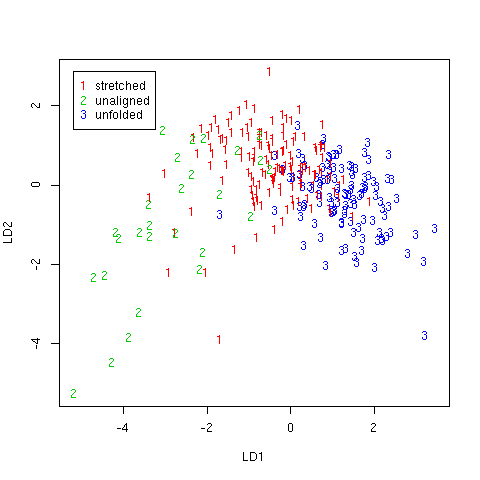
\includegraphics[width=1.1\textwidth]{figplotlda14.png}
  \caption{Plot of the two discriminant function values for the case with all 10  on-sheep traits plus density, IntGpDens, FollperGp, and FollGpArea, showing how the CrimpType groups separate}
  \label{fig:plotlda14}
\end{figure}

%\end{document}


This plot is very similar to the 10 trait case. 

We have to conclude that adding information about the spatial arrangement of follicles, at least in the form of IntGpDens, FollperGp, and FollGpArea, does little or nothing to improve classification.

As a last ditch attempt, we had a look at the ratio
\begin{eqnarray*}
IGDovFn & = & IntGpDens / Fn
\end{eqnarray*}
This measures the extent to which intra-group density exceeds overall follicle density. It varies from 0.5 to 2.5 with means as follows
\begin{verbatim}
  CrimpType  IGDovFn
1 stretched 1.141690
2 unaligned 1.348462
3  unfolded 1.168297
\end{verbatim}
so it might help separate the unaligned cases, but is not going to be much help in separating unfolded from stretched, which is the main problem. That is a little surprising as one would expect unfolded sheep to have the highest values for this ratio.
\end{document}

